\subsection{溶液的概念}

由两种或两种以上物质所组成的均匀混合体系称为溶液。广义的溶液包括气体溶液、液体溶液和固体溶液,溶液由溶质和溶剂组成。溶质和溶剂没有严格的定义,但通常把溶液中含量较多的那个组分称为溶剂。本章中所涉及的溶液是指溶剂为液体、溶质为固体的溶液。

许多物质在常温下是固体,但温度升到熔点以上时就熔化为液体。这种常温下是固态的纯物质的液相称为熔体。但在一般的应用中,通常把两种或两种以上在冷却时凝固的均匀液态混合物也称为熔体。例如液态的$\alpha$萘酚(熔点96℃)是熔体。$\alpha$萘酚和$\beta$萘酚(熔点122℃)的均匀液态混合物也称为熔体,但$\alpha$萘酚、$\beta$萘酚和乙醇的液体混合物却不能称为熔体,而应称为溶液了。

溶液和熔体,溶解和熔化,溶质和溶剂有时是很难严格区分的。例如KNO3在少量水的存在下,在远低于其熔点的温度下可化为液体,这样形成的液体就很难判断是溶液还是熔体,因为如果把它看成$\rm KNO_3$溶于水的溶液时,则溶剂又太少,如若称为水在$\rm KNO_3$中的溶液时也不符合习惯的叫法。在这种情况下,通常把该体系看作熔体,即$\rm KNO_3$“熔化”在少量的水中。

\begin{figure}[thpb]
 \centering
 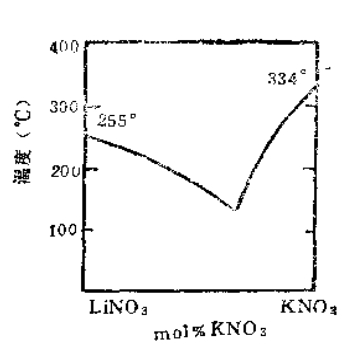
\includegraphics[width=0.5\textwidth]{fig/cp03/img3.1.jpg}
 \caption{$\rm LiNO_3-KNO_3$体系}
\end{figure}

\begin{figure}[thpb]
 \centering
 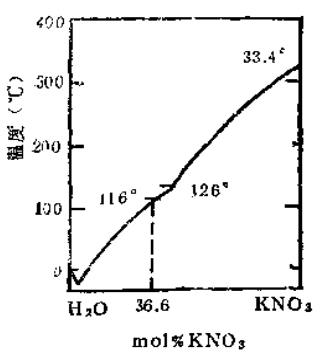
\includegraphics[width=0.5\textwidth]{fig/cp03/img3.2.jpg}
 \caption{$\rm H_2O-KNO_3$体系}
 (116℃是$\rm KNO_3$饱和溶液的沸点,126℃是$\rm KNO_3$的晶相转变温度)。
\end{figure}

如果从相图的观点来看问题,把溶液置于更广阔的范围内来讨论时,这些矛盾就可以统一起来了。例如在$\rm LiNO_3-KNO_3$体系的相图中(图3.1),低共熔点左右的两条液相线的范围是差不多的,都表示纯物质熔点因另一组分的加入而逐渐降低。该相图也可看成是溶解度图。此时,右边的曲线表示LiNO3在$\rm KNO_3$中的溶解度($\rm KNO_3$溶液);左边曲线则表示$\rm KNO_3$在LiNO3中的溶解度(LiNO3)。当状态点十分接近于$\rm KNO_3$熔点时(如成分为99.9\%的$\rm KNO_3$和0.1\%的LiNO3的样品在接近$\rm KNO_3$熔点(图3.1、图3.2)的温度下),LiNO3是液体,$\rm KNO_3$也在低于其熔点的温度下熔化。这种状态,一般认为是$\rm KNO_3$在少量LiNO3存在下熔化了,但也可以看成是999份$\rm KNO_3$溶解在1份LiNO3中。$\rm H_2O-KNO_3$体系的相图(图3.2)和$\rm LiNbO_3-KNO_3$体系是类似的。不同的是,其中一个组分,即H2O的熔点很低,左右两曲线的范围相差很大,但本质上没有什么差别。右边的曲线表示$\rm KNO_3$熔点因$\rm H_2O$的存在而下降的曲线,左边的曲线表示$\rm KNO_3$使$\rm H_2O$的冰点下降的曲线。由于$\rm H_2O$在常温下是液体,通常把右边曲线的下半部(图3.2中虚线左边,温度较低,含水量较多部分)看成$\rm KNO_3$在水中的溶解度曲线,而不是看成水使$\rm KNO_3$熔点降低的液相线。但在曲线的上部,我们虽然也可以把温度接近于$\rm KNO_3$熔点,含水量很少的液相(如含99.9\% $\rm KNO_3$,0.1\%$\rm H_2O$)看成是999份$\rm KNO_3$溶解在一份水中的溶液,但习惯上还是把这种情况看成$\rm KNO_3$在少量水的存在下熔化了。

由此可见,熔体和溶液是连续的,所以熔化和溶解在本质上是一样的。可以把熔化看成是被溶解所液化的特殊情况。当水是溶液的一个组分时,一般总是看成溶质(盐类)溶在一定温度的水中,而不是从水的存在使盐的熔点降低这个角度来看问题。习惯上把水多时称为溶解,而水很少时看成熔化。

